\documentclass[12pt, dvipsnames, a4paper]{article}
\usepackage{geometry}
\geometry{legalpaper, margin=0.5in}
\usepackage{xcolor}
\usepackage{lipsum,etoolbox}
\usepackage{xspace} 
\usepackage[normalem]{ulem}
\usepackage{vwcol}
\usepackage{cancel}
\usepackage{enumitem}
\usepackage{amsmath}
\usepackage{caption}
\usepackage{graphicx}
\usepackage{amsfonts}
\usepackage{float}
\usepackage{multicol}
\usepackage{hyperref}
\usepackage{listings}
\usepackage{textcomp}
\usepackage{lstautogobble}
\usepackage[parfill]{parskip}
\usepackage{tikz-qtree}
\usepackage{tikz}
\usepackage{hyperref}
\usepackage[english]{babel}
\usepackage[autostyle, english = american]{csquotes}
\MakeOuterQuote{"}
\usetikzlibrary{decorations.pathreplacing}
\tikzset{every tree node/.style={minimum width=4cm,draw,circle},
         blank/.style={draw=none},
         edge from parent/.style=
         {draw,edge from parent path={(\tikzparentnode) -- (\tikzchildnode)}},
         level distance=1.5cm}

%% Genearl %%
\renewcommand{\thesection}{\arabic{section}}


%% For convenience %%
\newcommand{\code}[1]{\texttt{#1}}
\newcommand{\bcode}[1]{\texttt{\textbf{#1}}}
\newcommand{\balert}[1]{\textbf{\alert{#1}}}
\newcommand{\rarrow}{$\Rightarrow$}
\newcommand{\tab}[1][0.5cm]{\hspace*{#1}}
\newcommand{\deepemphasis}[1]{\underline{\textbf{\Large{#1}}}}
\newcommand{\bfemph}[1]{\textbf{\emph{#1}}}
\newcommand{\OR}[0]{\lvert \: \rvert}

%% Colours %%
\definecolor{mLightBrown}{HTML}{EB811B}
\definecolor{mLightGreen}{HTML}{14B03D}

%% Pseudocode %% 
\lstdefinelanguage{pseudo}
{
	keywords=[1]{
		let,
		class,
		new,
		loop,
		until,
		end,
		if,
		else,
		then,
		return,
		while,
		for,
		to,
		fun,
		break,
		and,
		true,
		false,
		or,
		do,
		max,
		min,
		elif,
	},
	keywordstyle=[1]\color{black}\bf,
	keywords=[2] {
		invariant,
		precond,
		postcond
	},
	keywordstyle=[2]\color{blue}\bf
}

\lstset{
	breaklines		=	true,
	language 		= 	pseudo,
	basicstyle		=	\ttfamily,
	mathescape		=	true,
	escapeinside	=	||,
	tabsize			=	2,
	numbers			=	left,
	commentstyle	=	\color{OliveGreen},
	stringstyle		=	\color{mLightBrown},
	upquote			=	true,
	morestring		=	[b]',
	moredelim		=	[l][\rmfamily\itshape]{@},
	comment			=	[l]{//},
	morecomment		=	[s]{/*}{*/},
	commentstyle=\color{Gray}\ttfamily,
	showstringspaces=	false,
	showtabs		=	false,
	autogobble
}

%% Other %%
\setcounter{secnumdepth}{5}
\setcounter{tocdepth}{5}

% \patchcmd{<cmd>}{<search>}{<replace>}{<success>}{<failure>}
\patchcmd{\abstract}{\titlepage}{\titlepage% Insert ToC-writing after starting a titlepage
  \addcontentsline{toc}{chapter}{Abstract}}{}{}
\setcounter{secnumdepth}{3}
\setcounter{tocdepth}{3}

% Keywords command
\providecommand{\keywords}[1]
{
  \small	
  \textbf{\textit{Keywords---}} #1
}


%**************************************************************************************************************%
%______________________________________________________________________________________________________________%
\begin{document}
\title{\textbf{EECS 4314 - Bit Theory\\Dependency Extraction Report}}
\date{\Large \today}
\author{
	\large \textbf{Amir Mohamad}\\ \small amohamad@my.yorku.ca\\\\
	\large \textbf{Arian Mohamad Hosaini}\\ \small mohama23@my.yorku.ca\\\\
	\large \textbf{Dante Laviolette}\\ \small dantelav@my.yorku.ca\\\\
	\large \textbf{Diego Santosuosso Salerno}\\ \small nicodemo@my.yorku.ca\\\\
	\large \textbf{Isaiah Linares}\\ \small isaiah88@my.yorku.ca\\\\
	\large \textbf{Joel Fagen}\\ \small joefagan@my.yorku.ca\\\\
	\large \textbf{Misato Shimizu}\\ \small misato1@my.yorku.ca\\\\
	\large \textbf{Muhammad Hassan}\\ \small furquanh@my.yorku.ca\\\\
	\large \textbf{Yi Qin}\\ \small aidenqin@my.yorku.ca\\\\
	\large \textbf{Zhilong Lin}\\ \small lzl1114@my.yorku.ca\\\\
	\large York University\\
}
\maketitle
\newpage
\hspace{0pt}
\vfill
\begin{abstract}
	Dependency extraction for source code is a critical task in software engineering which involves identifying and extracting software components from the repositories. It is a process of obtaining source code from compiled executables, and it is essential for reverse engineering, software analysis and debugging. We can find the relationships, including function calls, variable references, and inheritance relationships among different components in the system. We will be able to maintain the software architecture features. By achieving these features, we can minimize changes' impact and ensure the system is always scalable and maintainable. It will also help refactor the code by identifying the components that might need to change from different files. In the report, we will extract the source code from the FreeBSD operating system and find the relationships between the components inside the system, including Understand, srcML and our custom method. During the research process, we used two different techniques to get more precise results and better compare the three methods.
	Based on these techniques, the quantitative and qualitative helped to show more secrete about dependency extraction.
	After those processes, we successfully compared three extraction methods and summarized their advantages and limitations.
	\\\\
	\keywords{dependency extraction, Understand, SrcML, quantitative, qualitative}
\end{abstract}
\vfill
\hspace{0pt}
\newpage
\tableofcontents
\clearpage

\section{Introduction}
In the report, we will be analyzing dependency extraction in software architecture development. As software changes over time, the architecture might be changed a lot. The process of dependency extraction will be able to reconstruct the structure of the software architecture. Dependency extraction allows developers to understand the meaning of the code-based information better and can improve the accuracy of automated text analysis and processing.
Understand is a commercial software tool that supports many programming languages. It can generate different reports such as metrics, dependency, and call graphs by analyzing the source code from the software. After analysis of the source code, it will also create a dependency graph which shows the relationships between different components and entities inside the source code. These dependency graphs will give the developers a clear view of the effect of each component and how these components will work together.
The official website briefly and concisely explains the functionalities of srcML, which is an infrastructure for the exploration, analysis, and manipulation of source code and a lightweight, highly scalable, robust, multi-language parsing tool to convert source code into srcML. Compared to Understand, srcML is an open-source software system that provides a way to generate the source code in an XML format, and XML format can be easily analyzed and manipulated using other software tools by the developers. SrcML can use different programming languages as input, and SrcML captures both the syntax and semantics of the code. By analyzing the source code, srcML will depend on the code's structure, including the variables' names and types.

\subsection{Overview}
The report contains several parts. Firstly, we will discuss the derivation process of the three methods of extracting dependencies, and we will show the use cases and diagram. We will discuss three main extraction strategies we decide to use in the dependency extraction: understand, srcML and custom. Then, we will discuss the quantitative and qualitative analysis to explain the performance metrics. Before concluding, we will analyze the limitations of the techniques used and explained in the report.

\section{Dependency Extraction}
\subsection{Understand}
The first technique we used to extract dependencies of the FreeBSD kernel is using the Understand static code analysis IDE. We used it to analyze the FreeBSD source code and generate the extracted dependencies in \code{freebsd\_FileDependencies.csv} format. This CSV file is then converted to a \code{raw.ta} file using \code{csv-to-ta.pl} perl script. The rest of the process after the \code{Start A}, in figure 1, state is complete is the same as the assignment 2 iterative architectural decomposition. This process takes roughly over 3 hours to complete from start to end.

\subsection{SrcML}
The second technique we used to extract dependencies of the FreeBSD kernel is using the SrcML tool to convert our source code into xml and perform \code{xPath} queries. We used it to analyze the FreeBSD source code and generate the extracted dependencies in \code{freebsd\_FileDependencies.xml} format. Similarly, the rest of the process after the \code{Start A} state, is the same iterative process. The SrcML method uses an \code{xPath} query, \code{src:unit[@type='include']/@filename | cpp:include/cpp:file}, on the XML to extract the include dependencies. This method takes about 20 minutes for the entire process.


\section*{SrcML Introduction}

As part of our ongoing efforts to understand and analyze the FreeBSD kernel's structure, we have successfully extracted file-level dependencies using the srcML tool. we will outline the steps taken to achieve this goal and provide an overview of each step. Our findings helped us tremendously in understanding the kernel's architecture and identifying areas for optimization or improvement.

\section{Installing and Configuring srcML}

we installed the srcML tool on our local machines. srcML is an open-source tool designed to convert source code into an XML format, which makes it easier to analyze and manipulate using XPath queries. After installing srcML, we familiarized ourselves with its documentation and basic usage, enabling us to use it effectively in the next steps.

\section{Converting the FreeBSD Kernel Source Code to XML}

With srcML installed and configured, we proceeded to convert the entire FreeBSD kernel source code into an XML format. Using the command:

\begin{verbatim}
srcml freebsd/src/sys -o freebsd_kernel.xml
\end{verbatim}

we directed srcML to process the source code located in the \texttt{freebsd/src/sys} directory and output the resulting XML to a file named \texttt{freebsd\_kernel.xml}. This step was essential for enabling us to perform XPath queries on the source code data.

\section{Extracting Include Units and Files with XPath}

Now that we had the kernel source code in XML format, we used an XPath query to extract all the include units and their respective files. We executed the following command:

\begin{verbatim}
srcml freebsd_kernel.xml --xpath="//src:unit[@type='include']/@filename | //cpp:include/cpp:file"
\end{verbatim}

This XPath query searched for all \texttt{src:unit} elements with a \texttt{type} attribute set to \texttt{include}, as well as all \texttt{cpp:include/cpp:file} elements. The query then returned the \texttt{filename} attribute of each matching element. This step provided us with a comprehensive list of all the included files and their dependencies.

\section{Generating a Raw TA File}

With the data extracted, we created a custom script to parse the output from the previous step and generate a raw TA file.  Our custom script iterated through the list of include units and files, reformatting the data into the desired format and outputting it to the raw TA file.

\section*{srcML Conclusion}

In conclusion, we have successfully extracted file-level dependencies within the FreeBSD kernel using the srcML tool and a series of XPath queries. srcML has some limitations that users should be aware of when using it for source code analysis. it can be computationally intensive and time-consuming when processing large codebases, potentially impacting the efficiency of the analysis. Finally, srcML's XML output can be cumbersome to work with and may require additional tools or expertise to manipulate and analyze effectively, However, being efficient in XPath Queries can help save time in writing multiple lines of code.

\subsection{Custom Script}
The last technique we used to extract dependencies of the FreeBSD kernel is using a custom script to recursively scan our source code and match include directives with regex. This is all done in our \code{gen-ta-file.py} script. We used this script to generate the \code{freebsd\_FileDependencies.raw.ta} file without any intermediate tools. Similarly, the rest of the processes after the \code{Start A} state is complete, is the same iterative process mentioned earlier. This method is the fastest of the three since it does not have intermediate steps for \code{Start A} state. It takes about 10 minutes.

\subsection{Diagrams}
Figure 1, 2, and 3 below are a more detailed overview of the derivation process of each dependency extraction method.
\begin{figure}[!htb]
	\center
	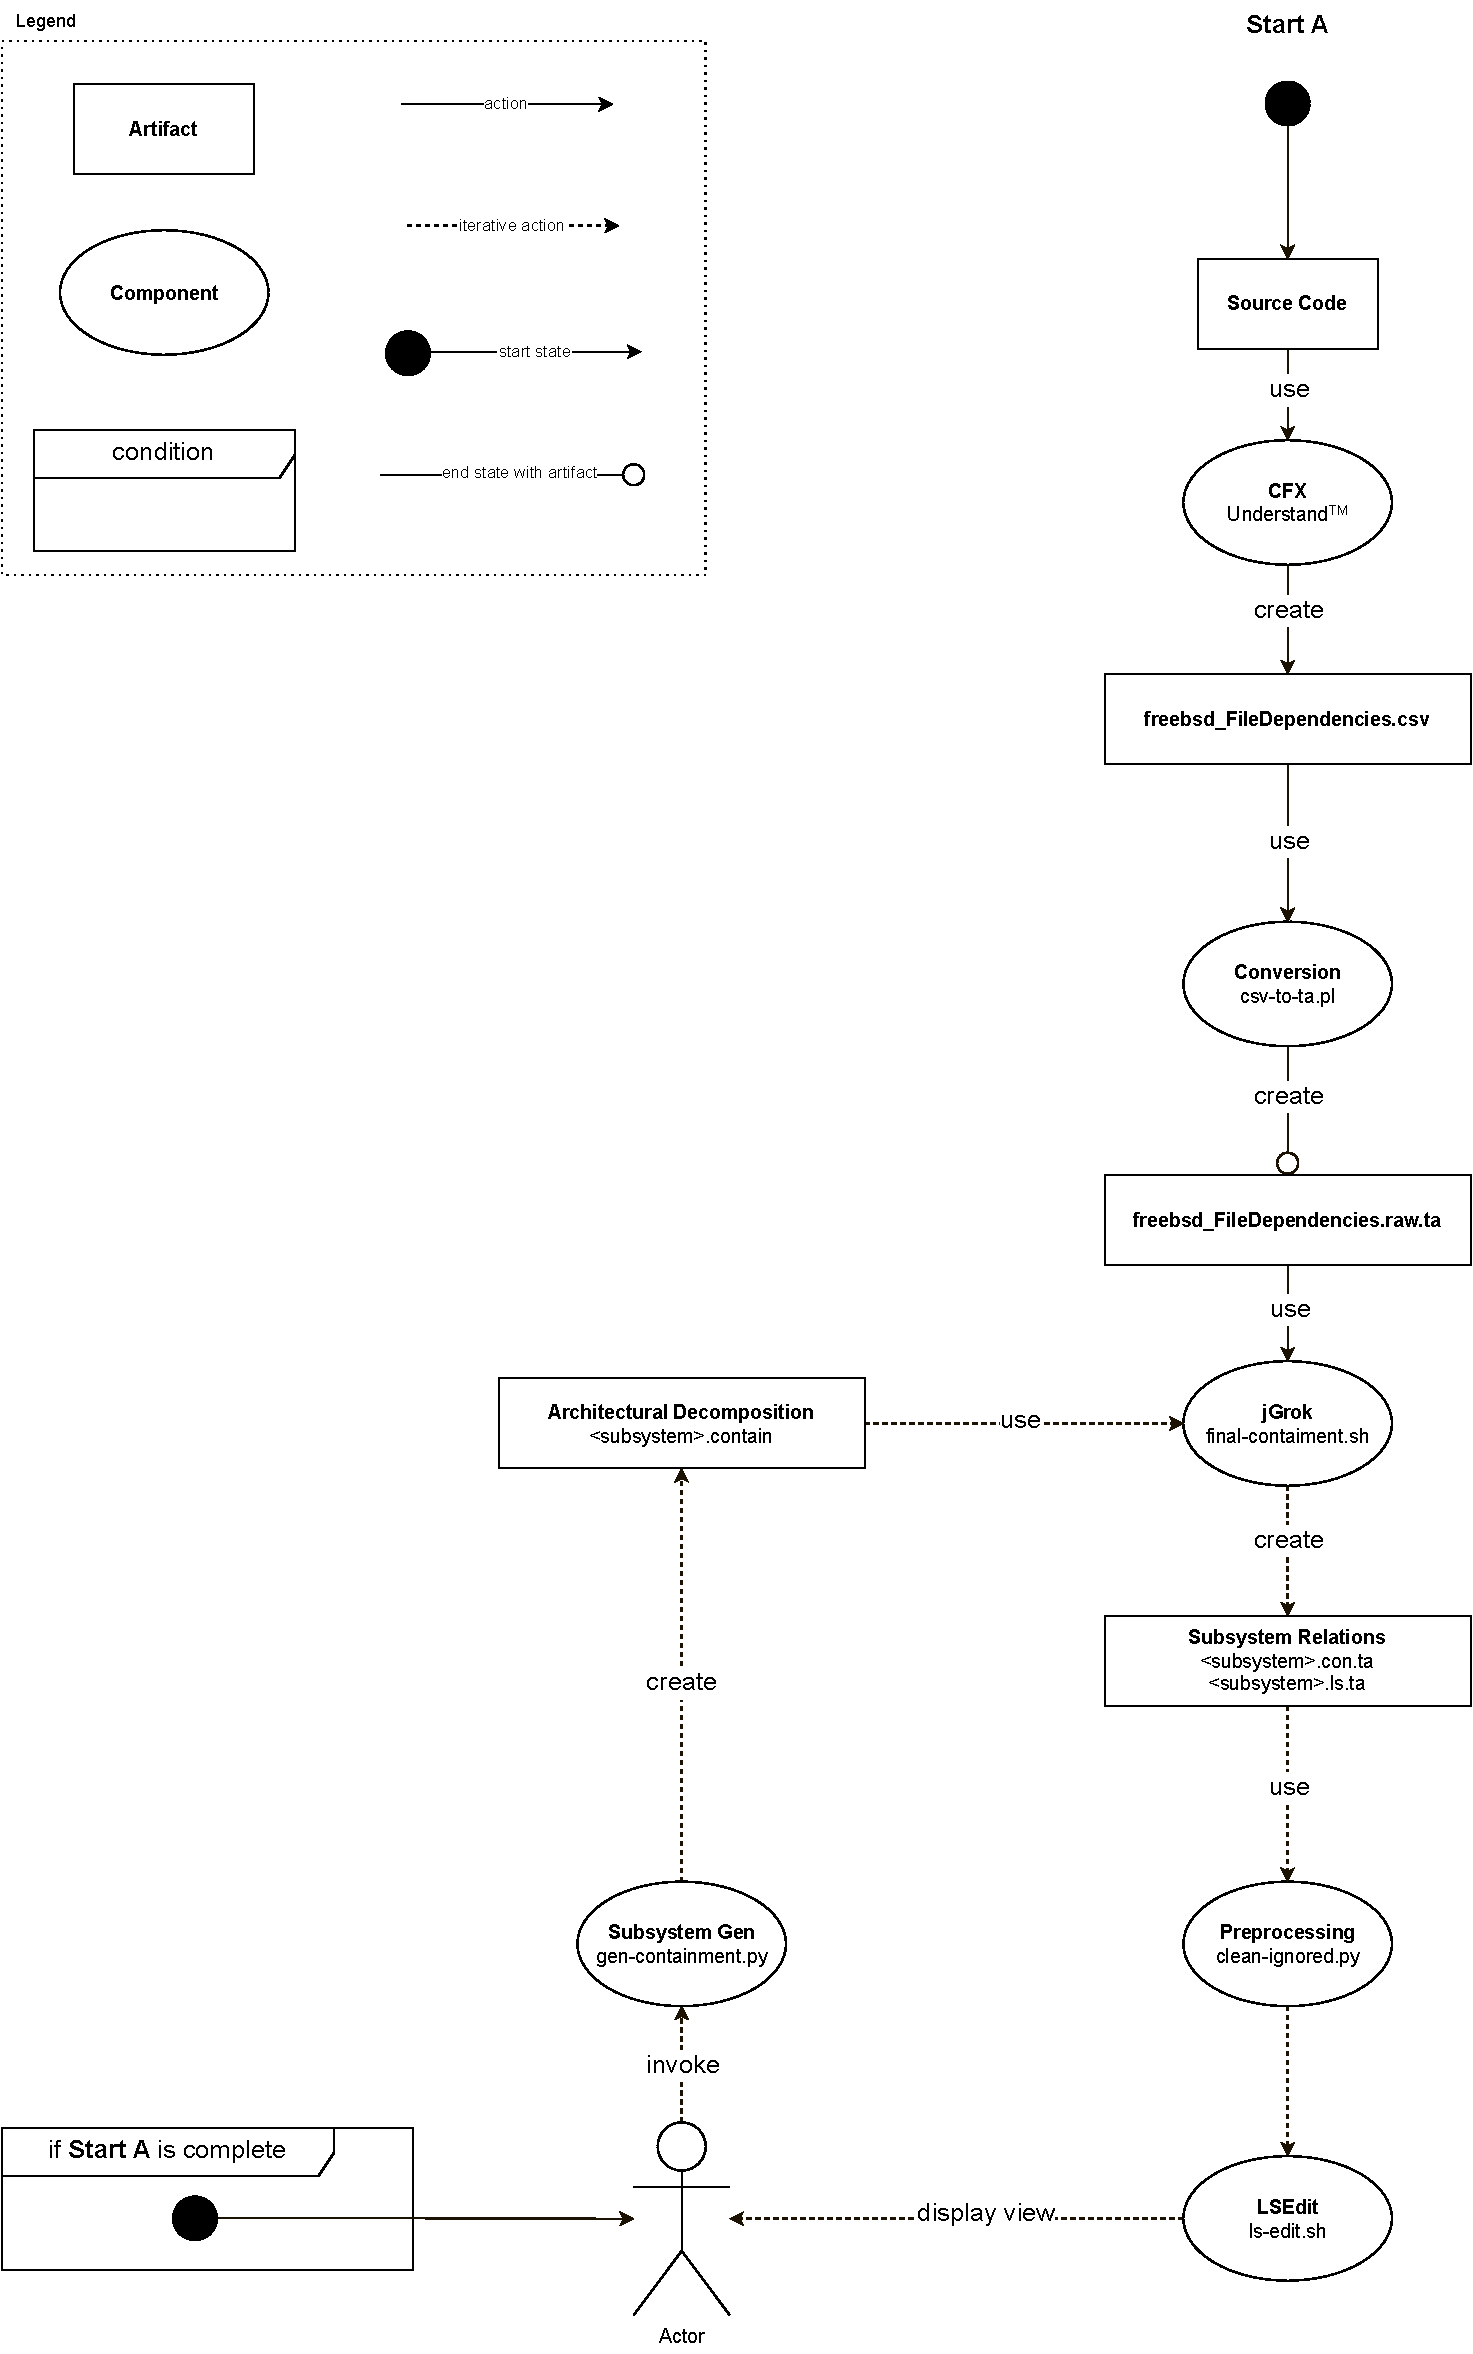
\includegraphics[width = 250pt]{assets/derivation/understad.pdf}
	\caption{Understand dependency extraction derivation process.\cite{understand}\cite{sourcecode}}
\end{figure}
\begin{figure}[!htb]
	\center
	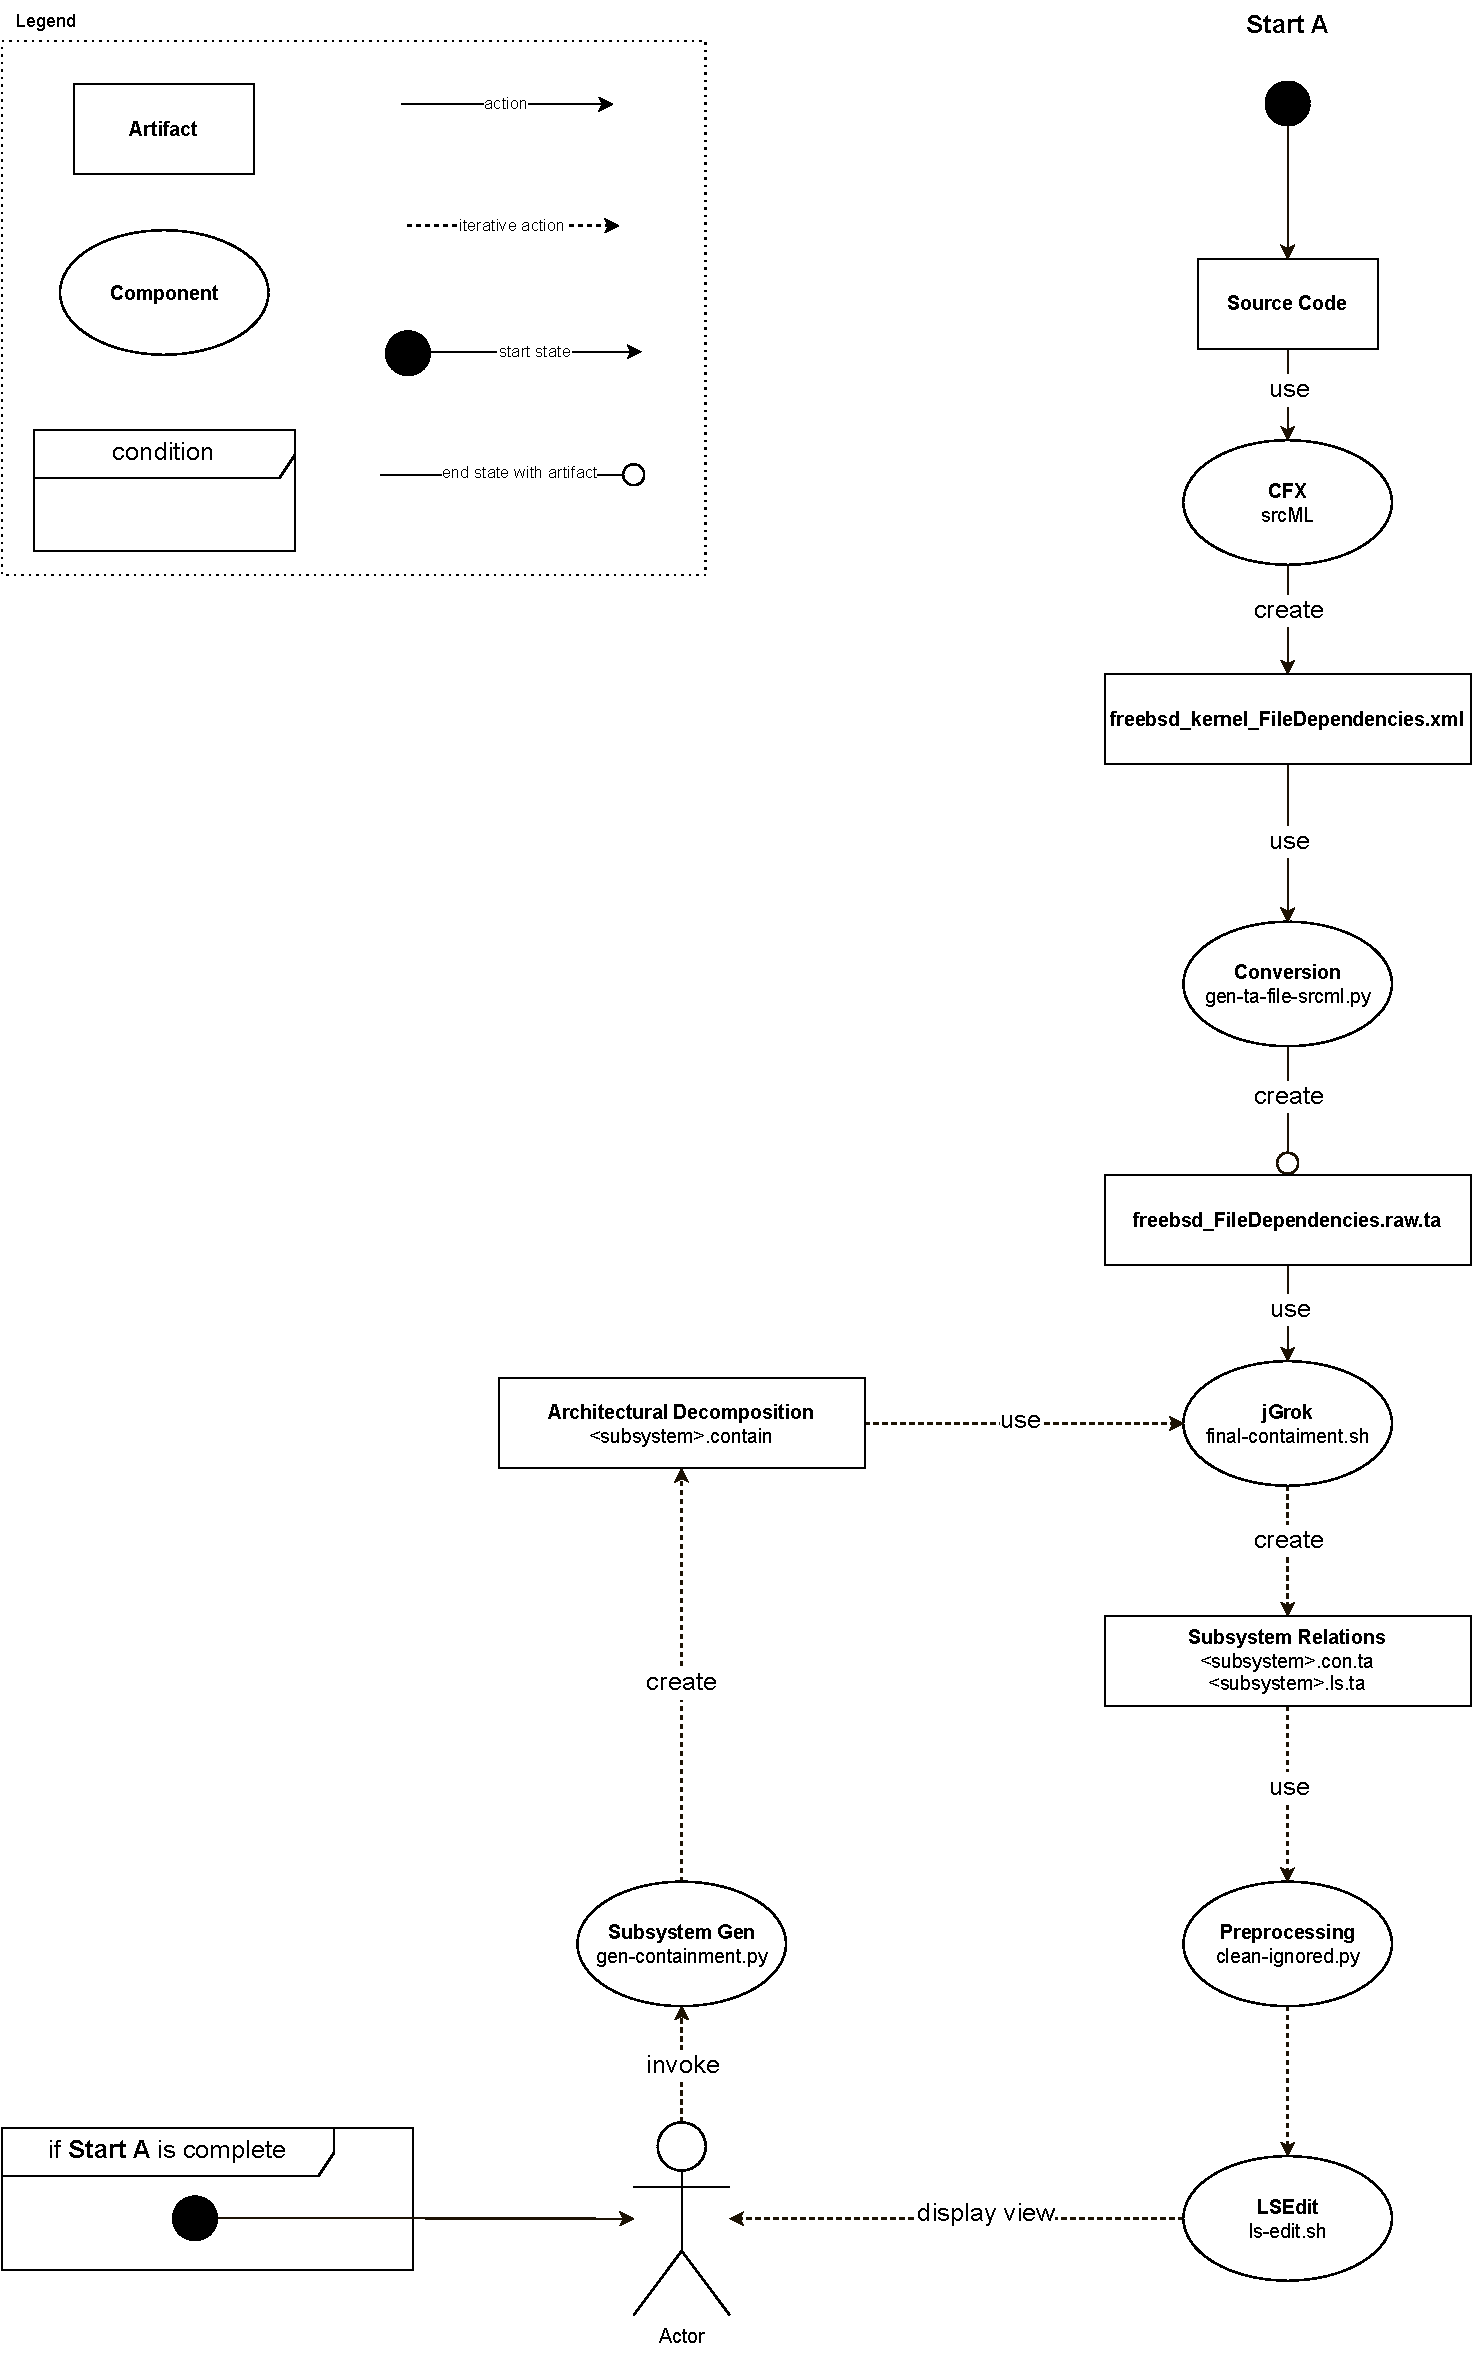
\includegraphics[width = 250pt]{assets/derivation/srcml.pdf}
	\caption{SrcML dependency extraction derivation process. \cite{sourcecode}}
\end{figure}
\begin{figure}[!htb]
	\center
	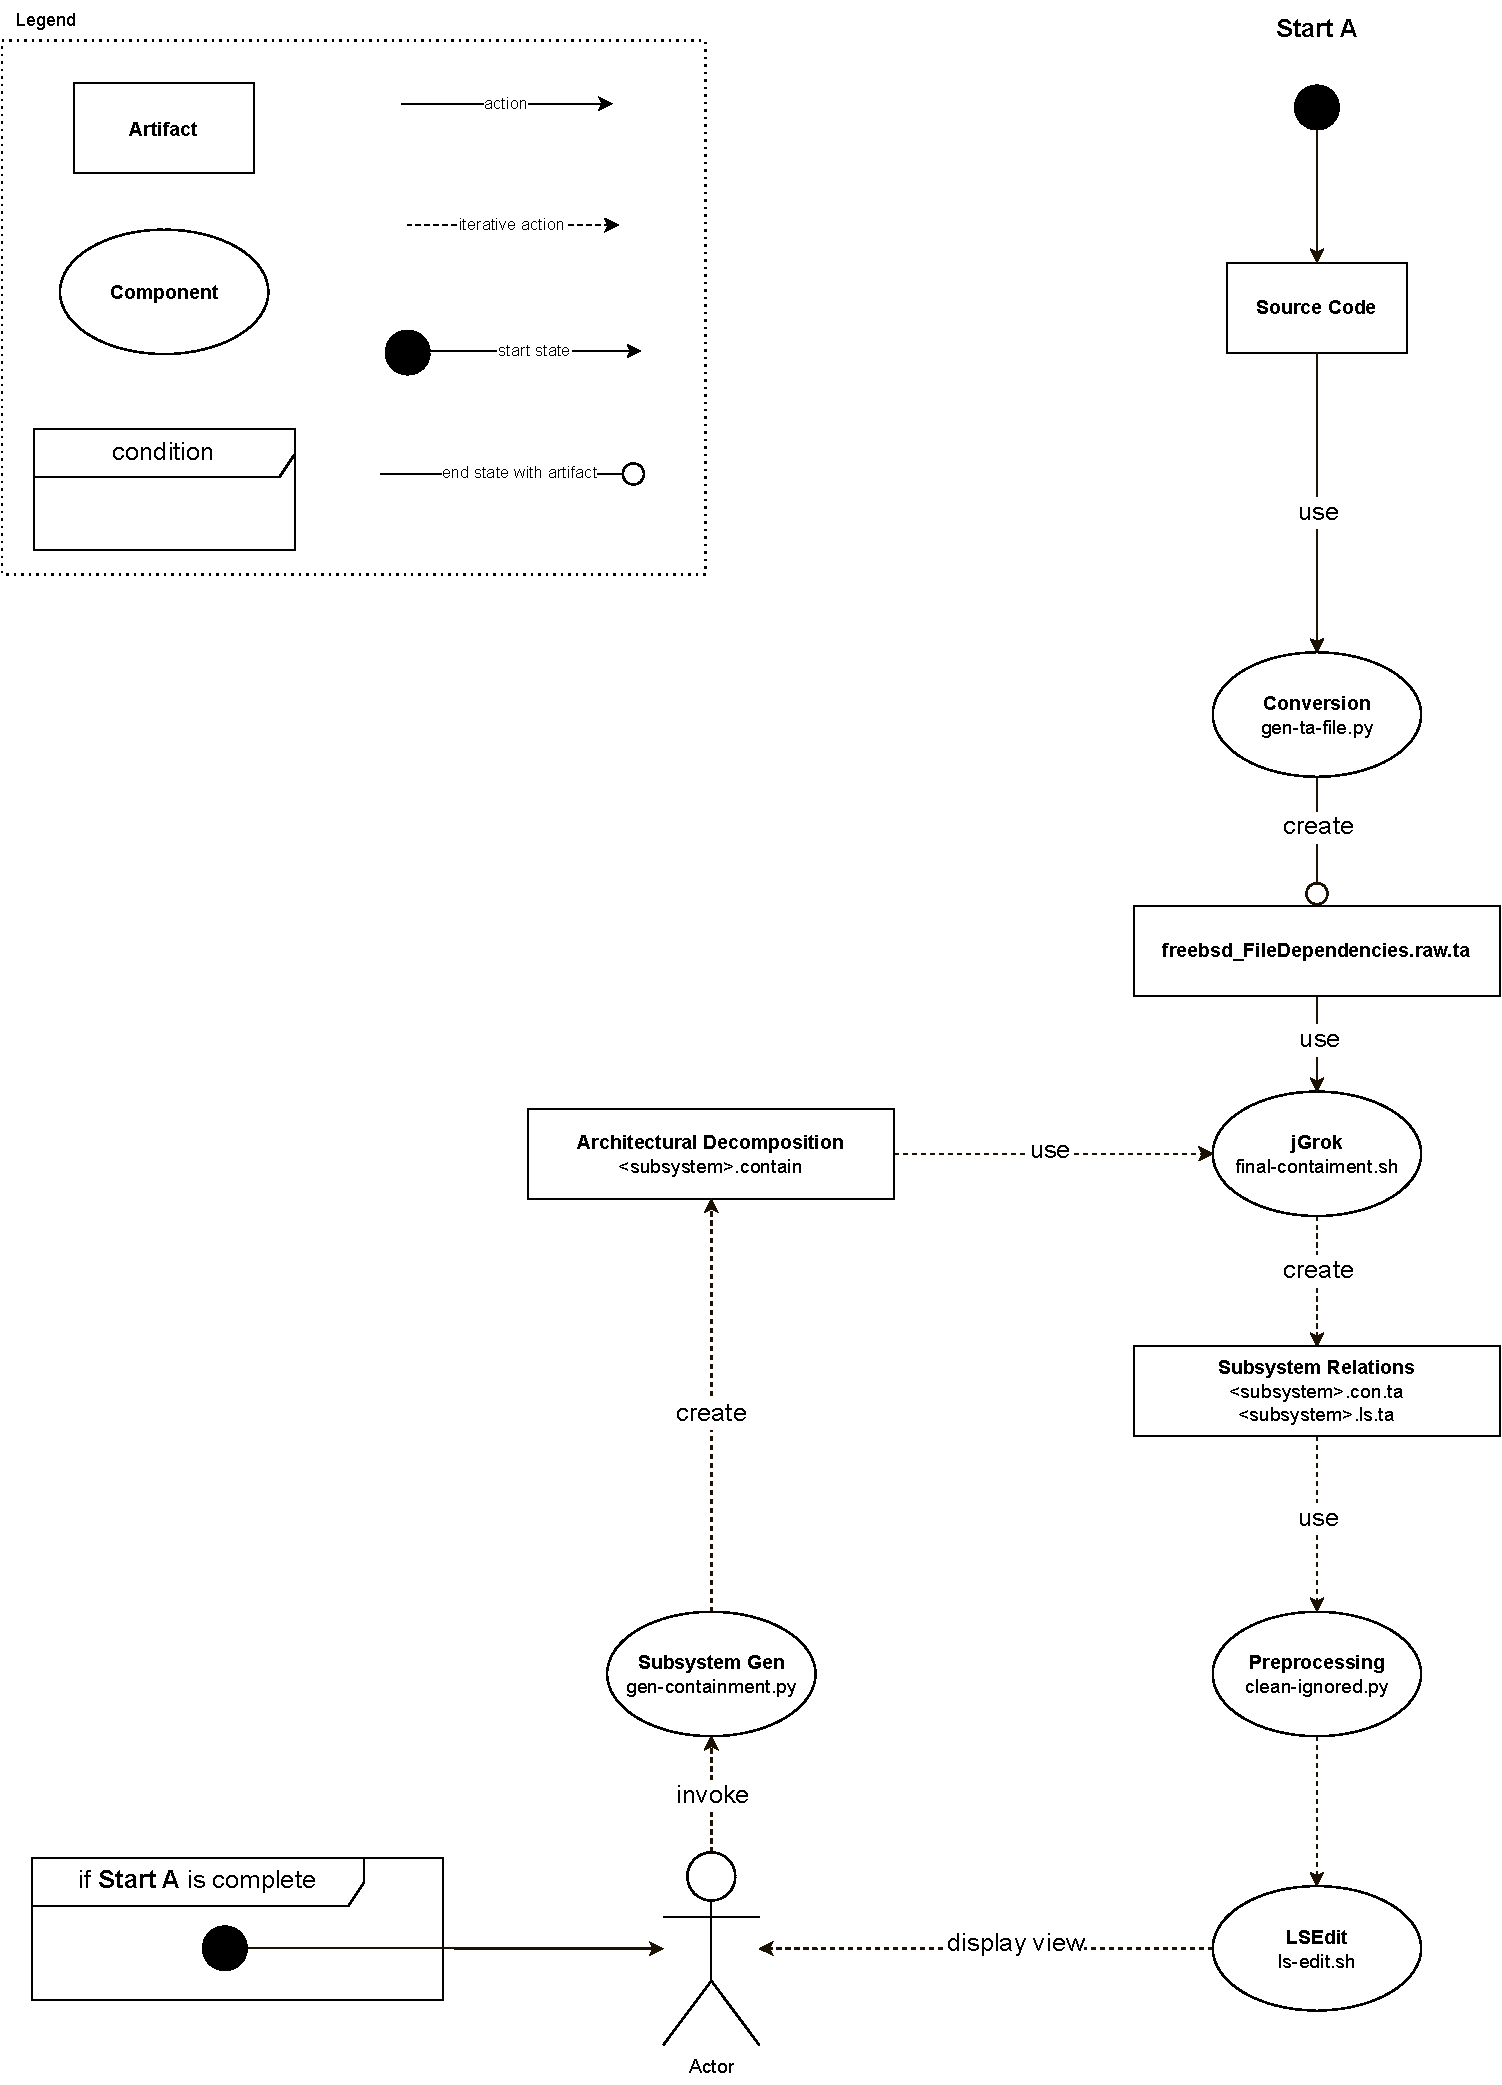
\includegraphics[width = 350pt]{assets/derivation/custom.pdf}
	\caption{Custom dependency extraction derivation process.\cite{sourcecode}}
\end{figure}


\clearpage
\subsection{Generation of Raw TA Files}
The main difference between our various dependency extraction processes
is the generation of the \texttt{*.raw.ta} file. Once this file has been generated,
the processes generally follow the same steps. With that being said,
the following diagrams show how the \texttt{*.raw.ta} files are generated
in our 2 custom methods.
\begin{figure}[!htb]
	\center
	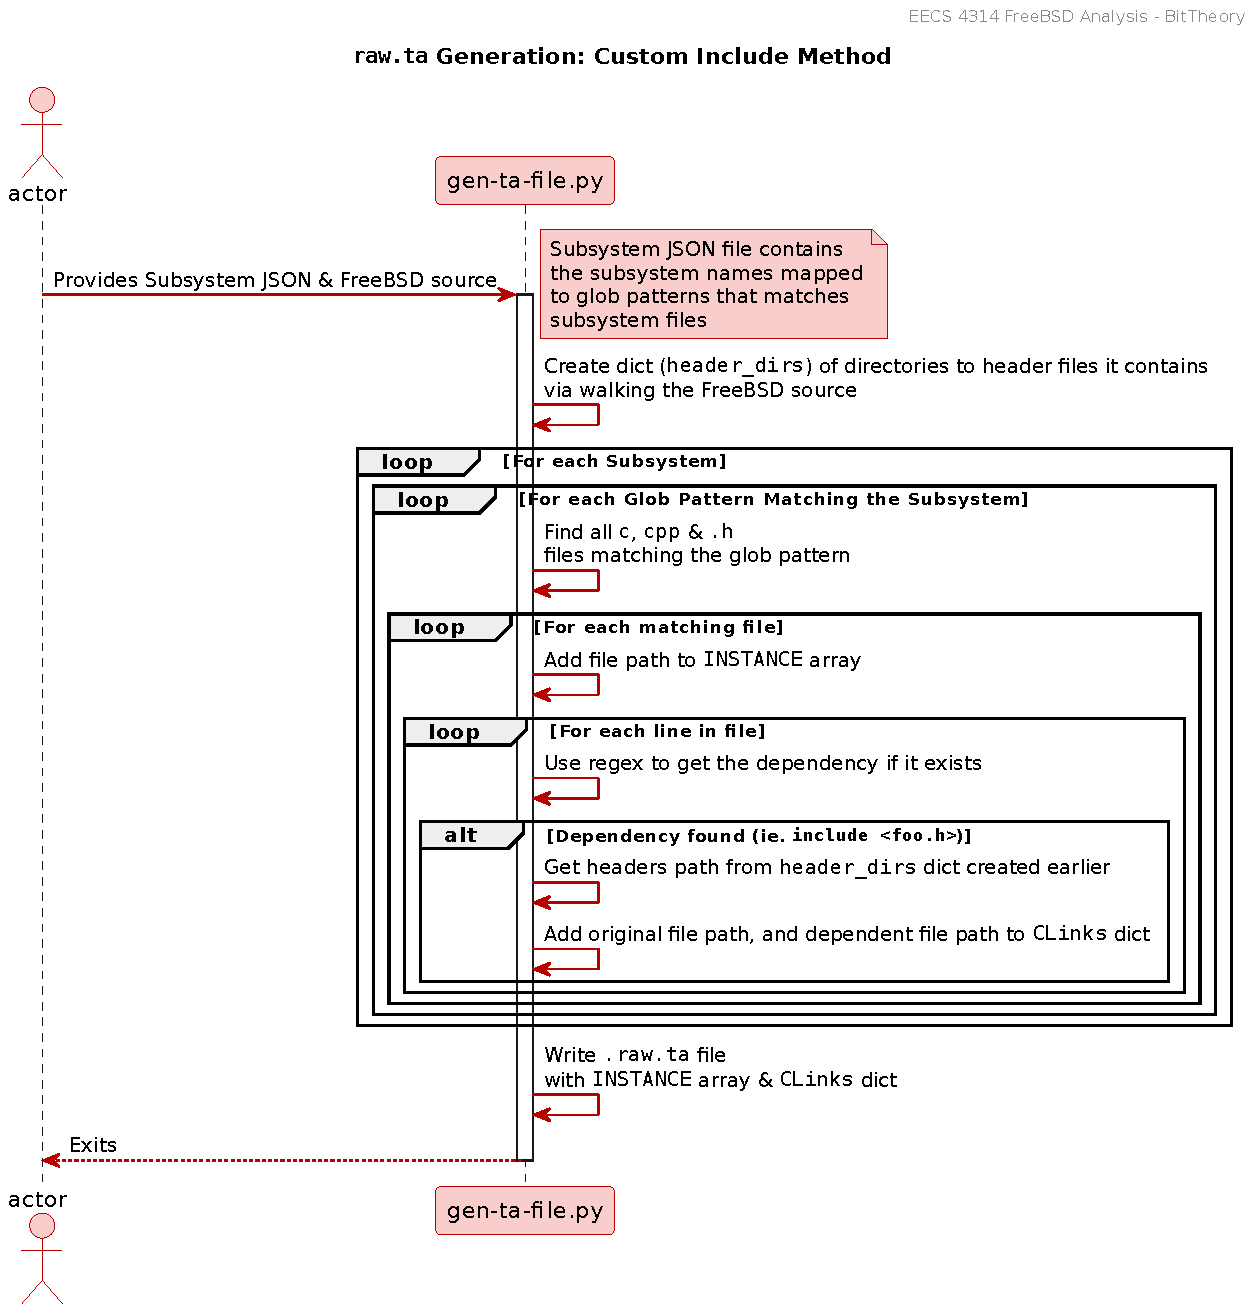
\includegraphics[width = 350pt]{assets/sequence_diagrams/custom_includes.pdf}
	\caption{Raw TA file generation using custom includes script.\cite{sourcecode}}
\end{figure}

\begin{figure}[!htb]
	\center
	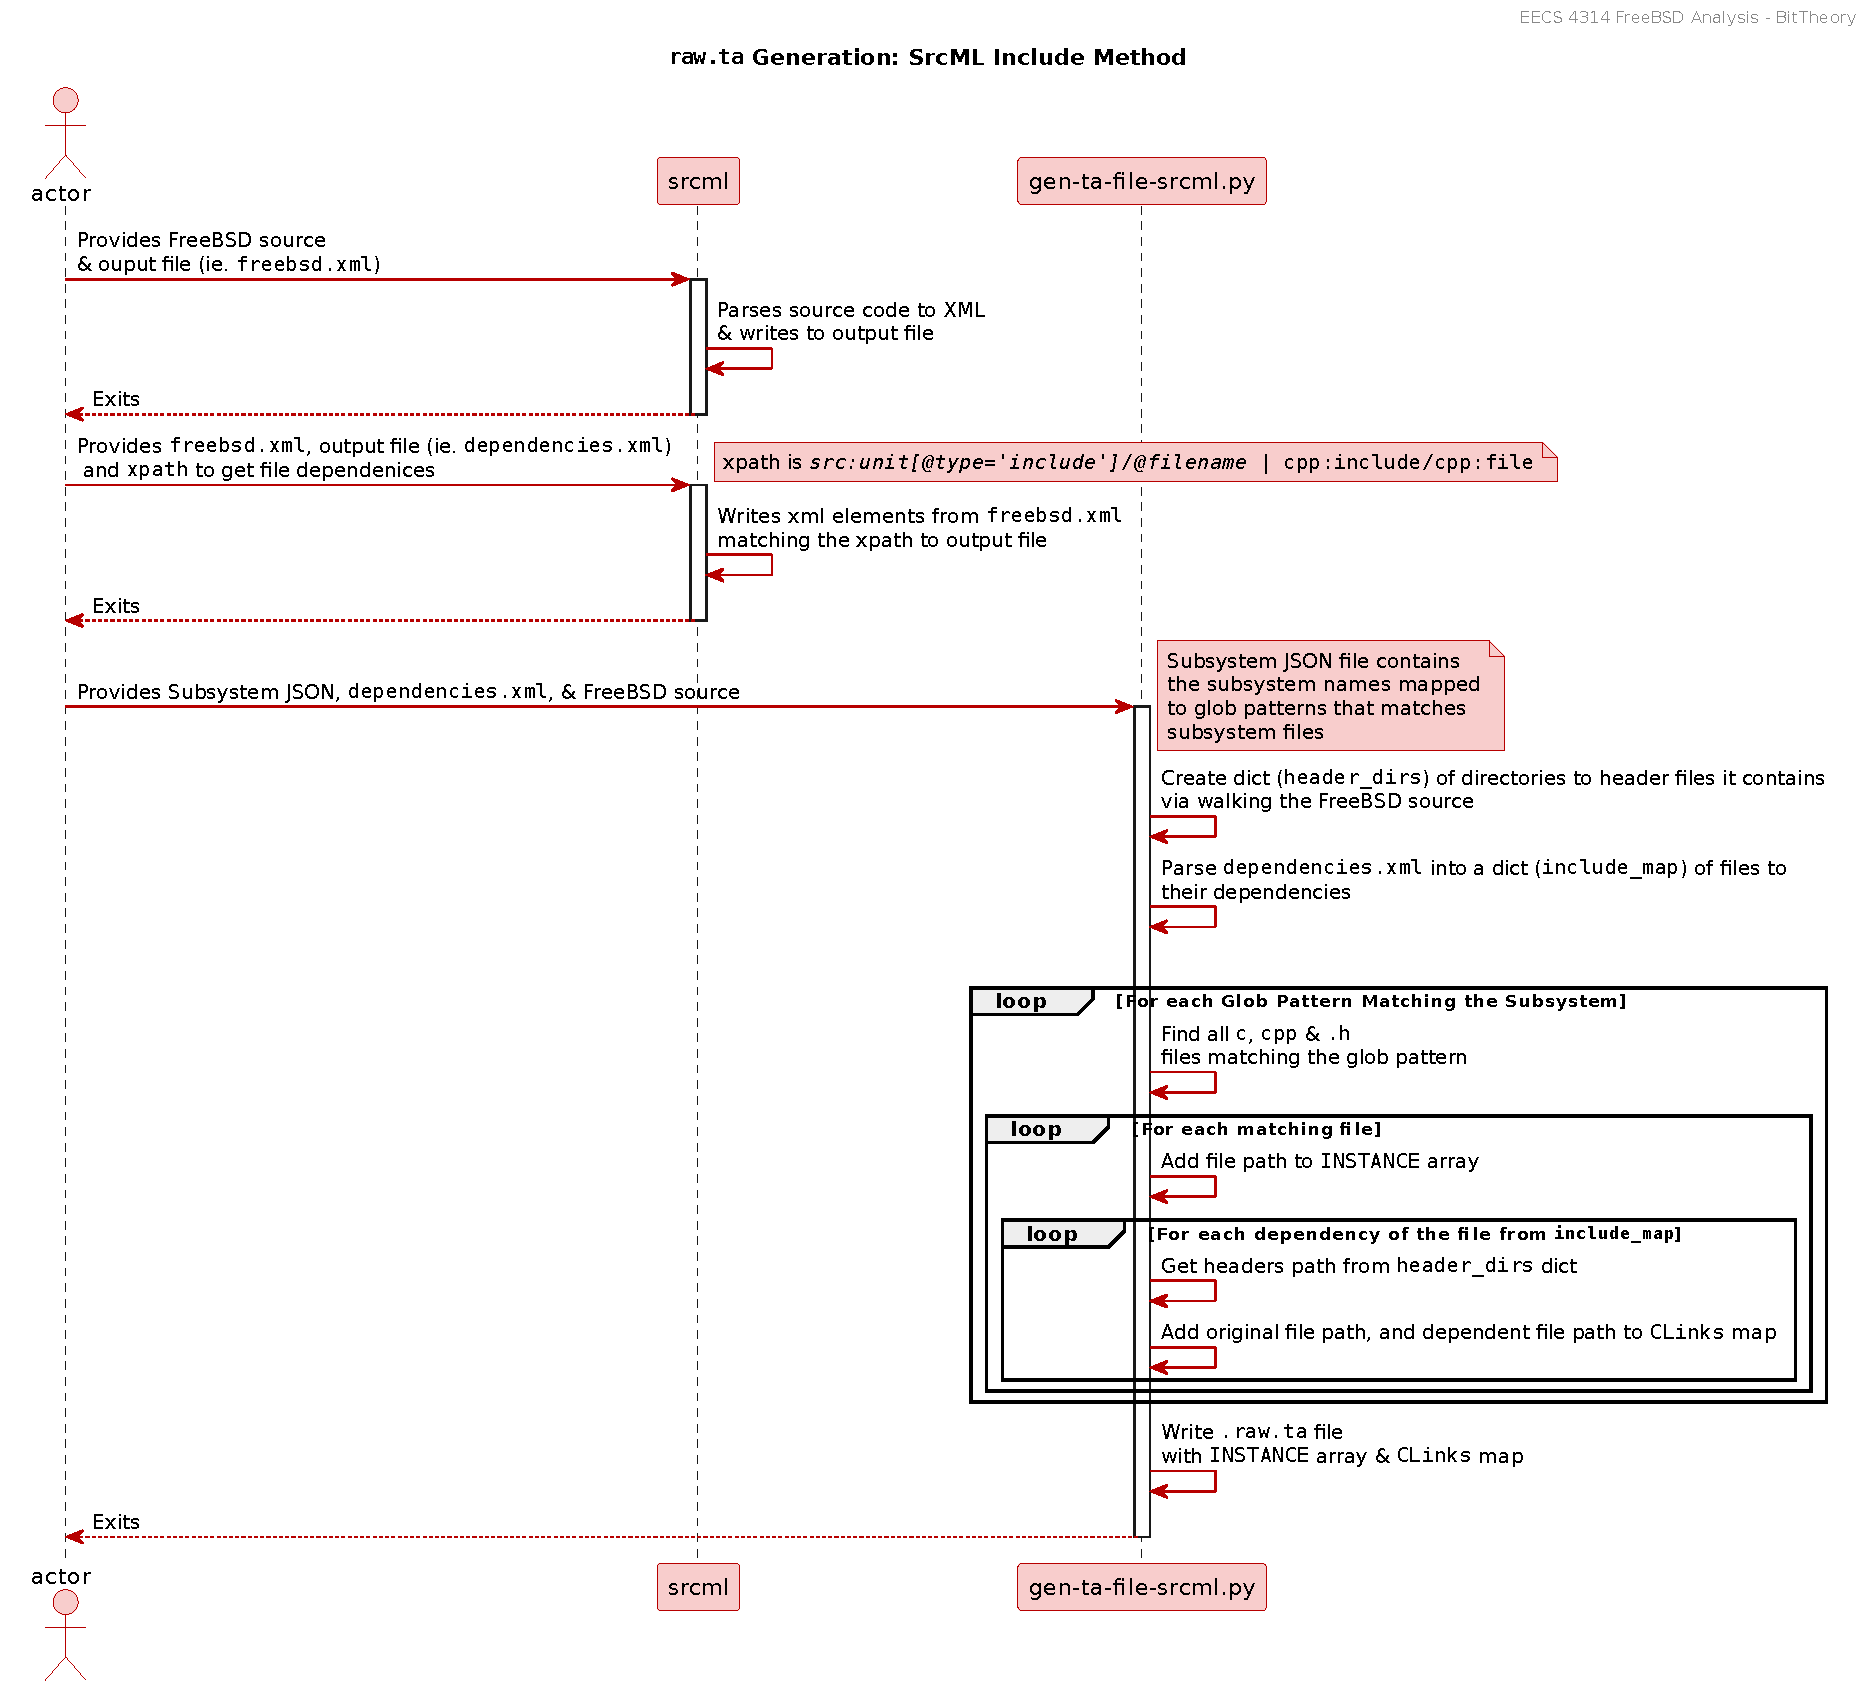
\includegraphics[width = 450pt]{assets/sequence_diagrams/srcml_includes.pdf}
	\caption{Raw TA file generation using custom SrcML script.\cite{sourcecode}\cite{srcml}}
\end{figure}

\section{Quantitative Analysis}
\subsection{Process of Quantitative Analysis}

We used a python script \code{gen-statistics.py} in order to generate our results for this analysis. This script would take 3 \code{ls.ta} extraction files for each tool that we implemented in this project, then read every line from each extraction file looking for \code{cLinks} dependencies. The script then adds the dependencies to a respective set for each tool using the “from file” and “to file” as a key. Then we use python set theory functions to find useful statistics such as: the size of the intersection between each two tool dependency sets, the size of the intersection of all dependency sets, the size of the exclusive dependency set for each tool, and the size of the union of all dependency sets. Finally this information is logged into a txt file for future reference. Finally we use this file to generate the following visualizations.

\subsection{Direct Comparison}

\begin{figure}[H]
	\center
	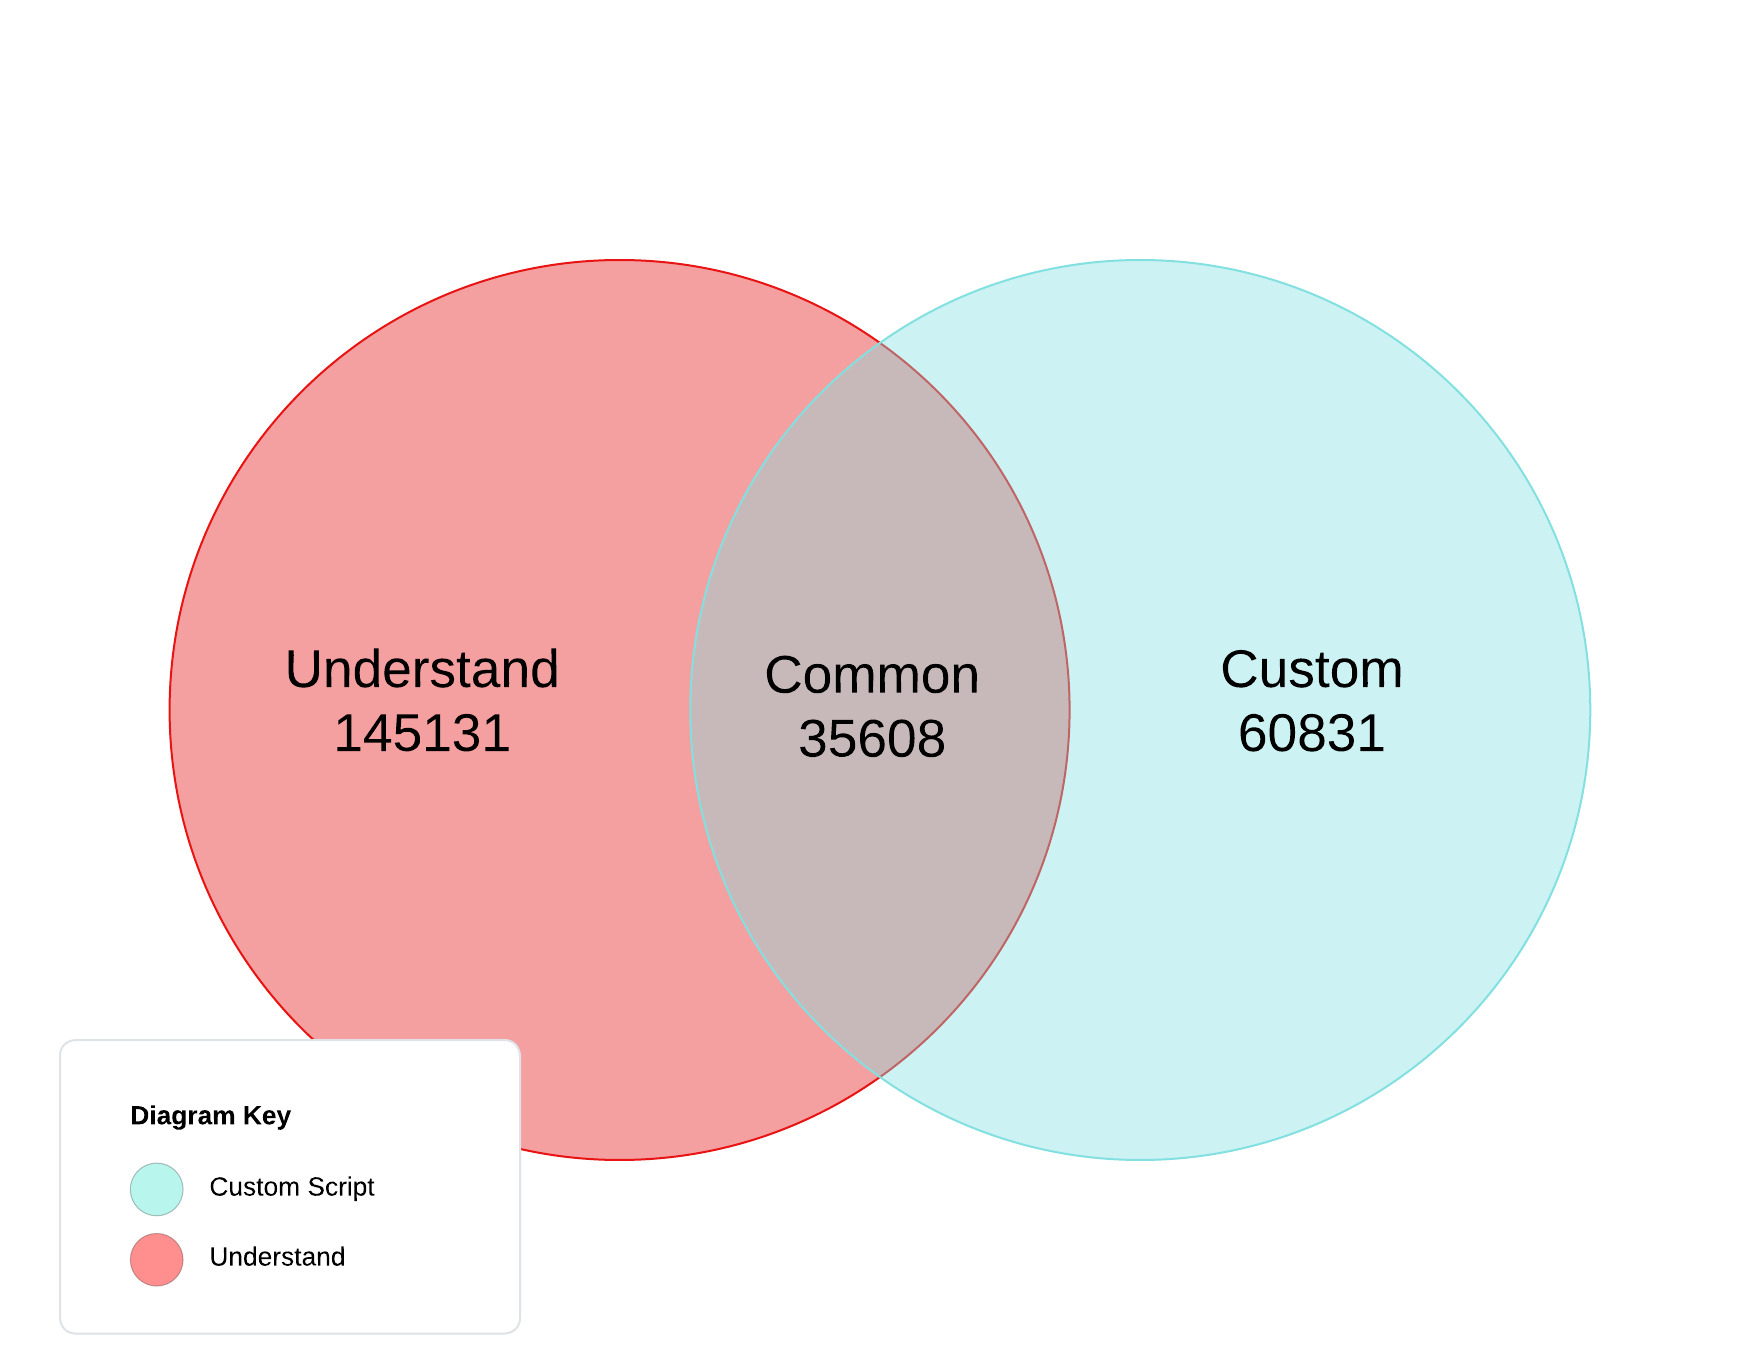
\includegraphics[width = 290pt]{assets/UnderstandCustom.jpeg}
	\caption{Direct comparison between the number of dependencies found from the Understand extraction tool and the Custom "include" extraction}
\end{figure}

\begin{figure}[H]
	\center
	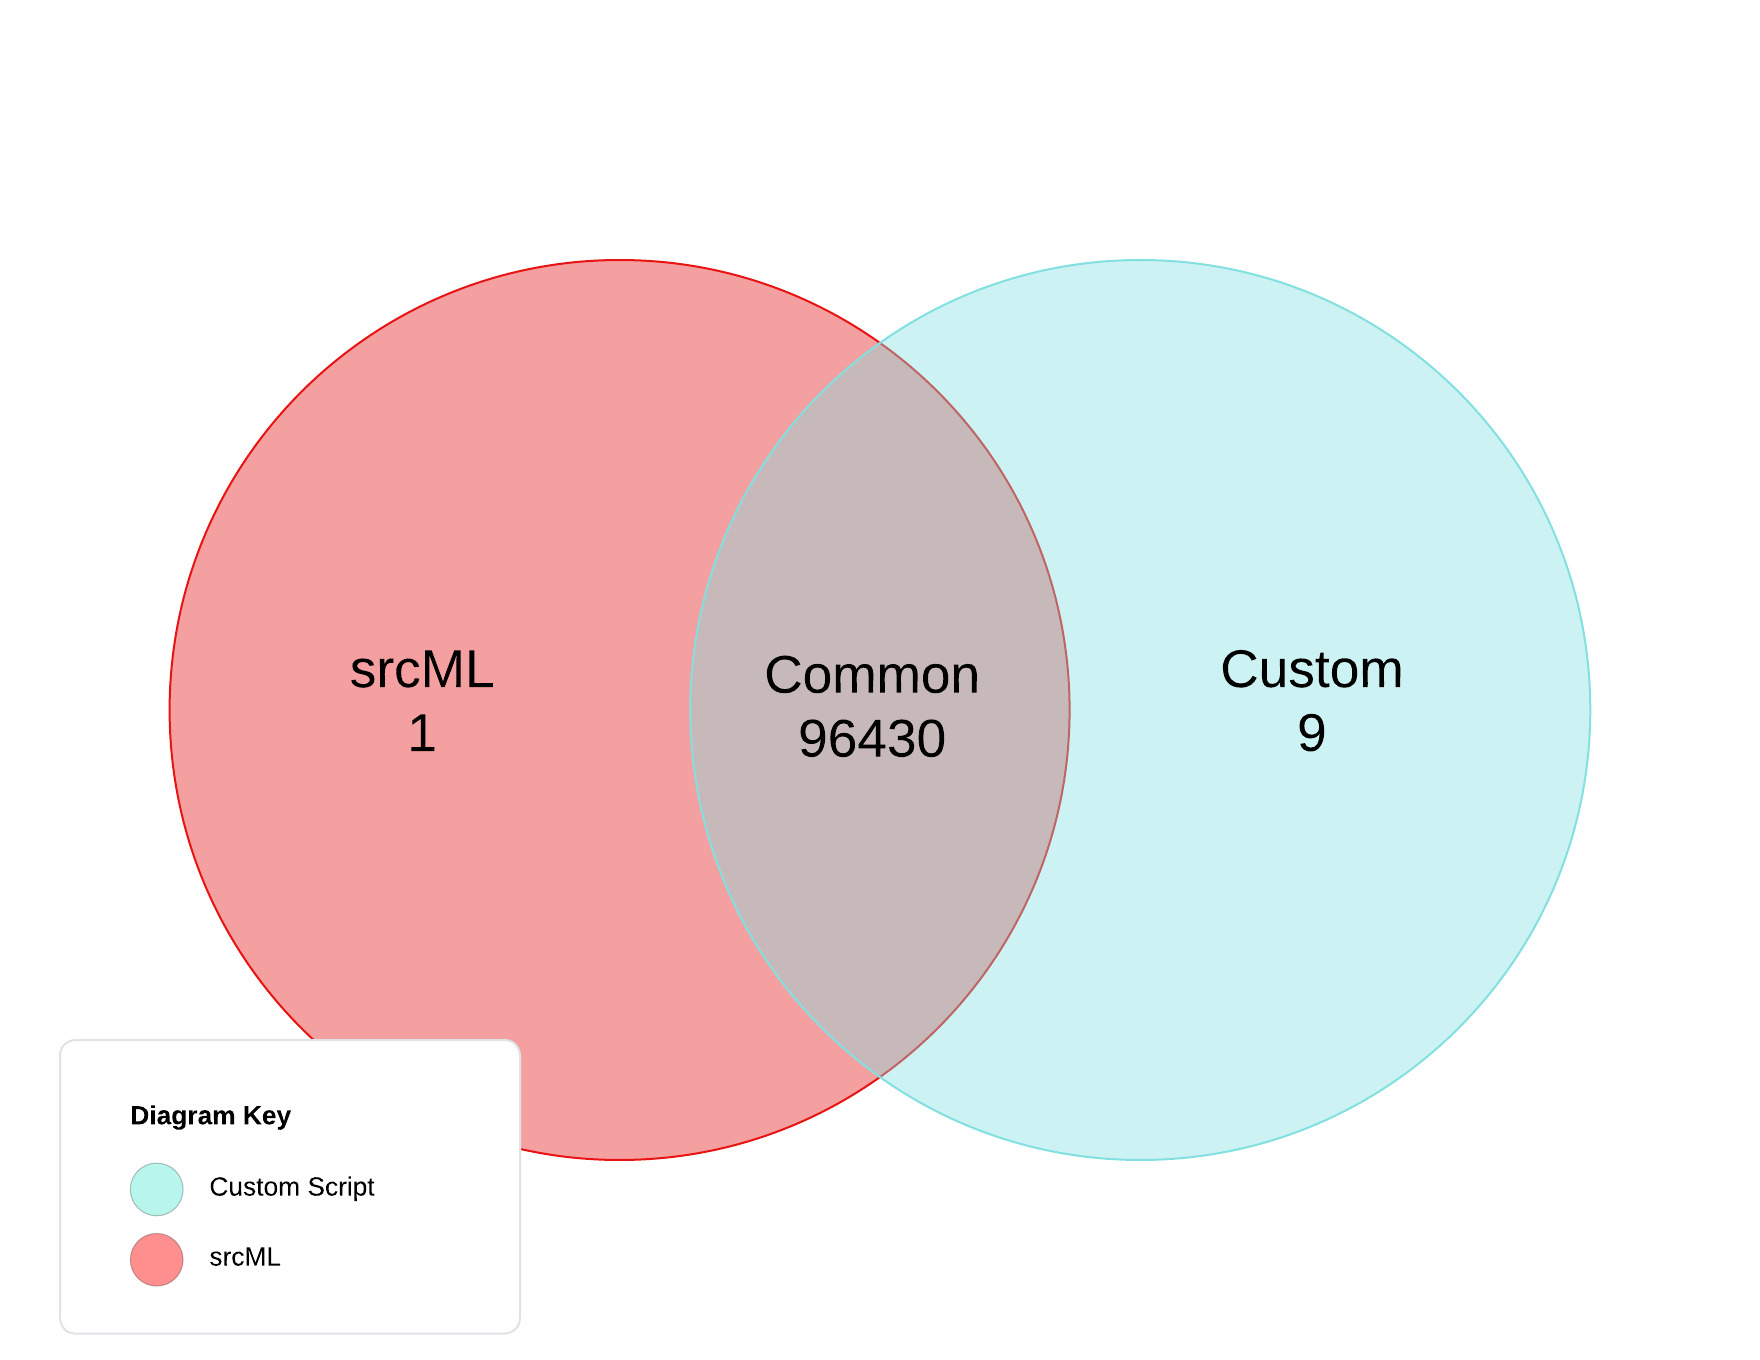
\includegraphics[width = 290pt]{assets/srcMLCustom.jpeg}
	\caption{Direct comparison between the number of dependencies found from the srcML extraction tool and the Custom "include" extraction}
\end{figure}

\begin{figure}[H]
	\center
	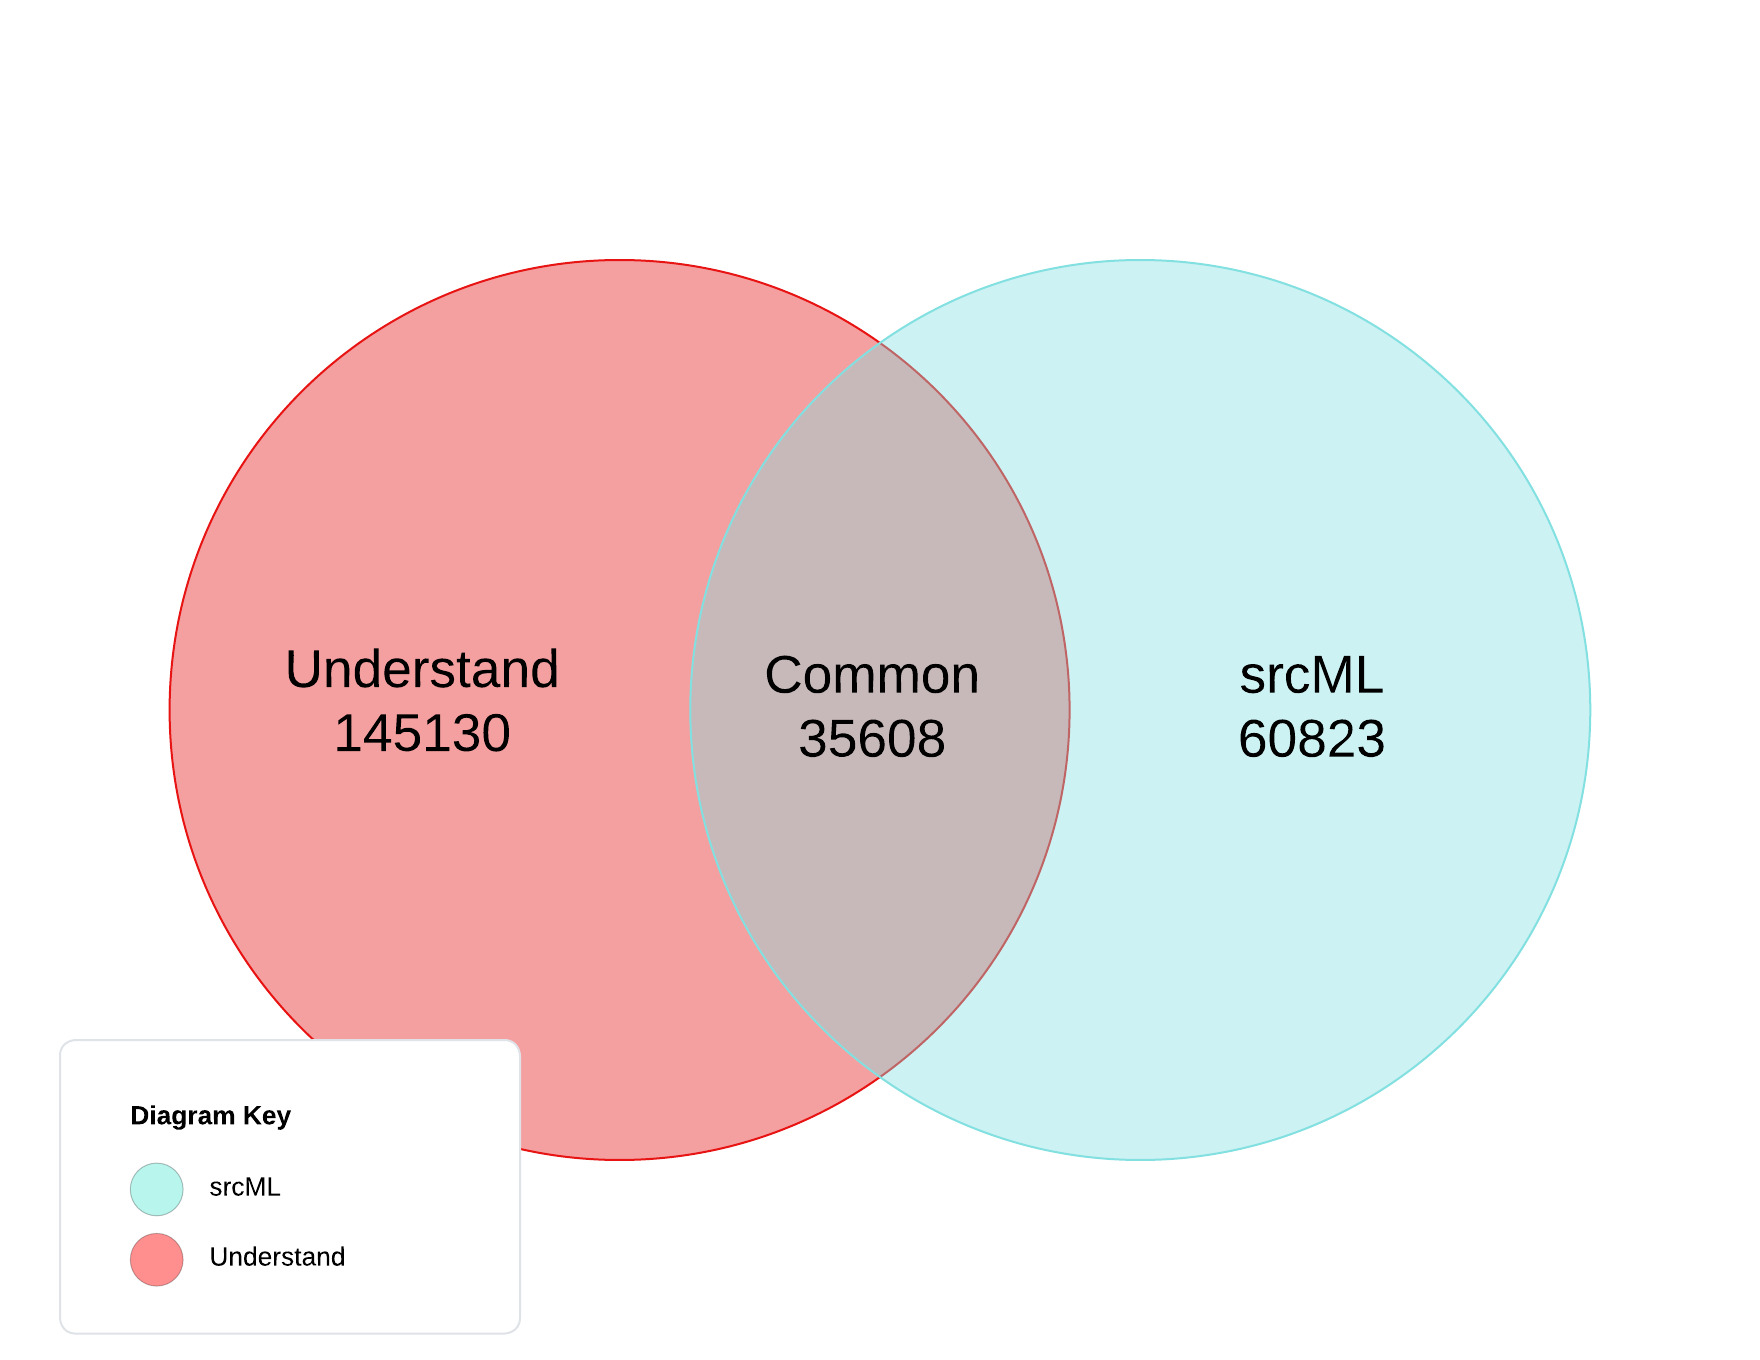
\includegraphics[width = 290pt]{assets/UnderstandSrcML.jpeg}
	\caption{Direct comparison between the number of dependencies found from the Understand extraction tool and the scrML extraction tool}
\end{figure}

\subsection{Quantitative Analysis Table}
\begin{tabular}{ |p{6cm}||p{6cm}|p{5cm}|  }
	\hline
	\multicolumn{3}{|c|}{Number of dependencies}                                                    \\
	\hline
	Extraction Tool                  & Total number of dependencies & Number of unique dependencies \\
	\hline
	Understand                       & 180,739                      & 145,130                       \\
	srcML                            & 96,431                       & 1                             \\
	Custom Script                    & 96,439                       & 9                             \\
	$Understand \cap  srcML$         & 35,608                       & 1                             \\
	$Understand \cap  Custom Script$ & 35,608                       & 1                             \\
	$srcML \cap Custom Script$       & 96,430                       & 60823                         \\
	All three (union)                & 241,570                      & N/A                           \\
	All three (common)               & 35,607                       & N/A                           \\
	\hline
\end{tabular}
\newline
\newline
\\
\\
The above table above shows the number of dependencies extracted from each extraction tool. Understand has the most dependencies out of the three extraction tools, with 180,739 dependencies total. If we divide the number of unique dependencies of Understand by its total number of dependencies, we get $($$145130 \div 180739$$) \approx 80\%$. From this we can conclude that 80\% of Understand's extracted dependencies are unique to that tool.
\newline
One observation was that Understand was able to extract far more unique dependencies than srcML and our custom script put together. Combined, $srcML \cap Custom Script$ extracted 60,823 unique dependencies, but Understand managed to extract 145,130 dependencies, which is more than double. The srcML by itself only captured one unique dependency, and our custom script only captured 9 unique dependencies, compared to the large number that Understand gathered.
\newline
One thing to note is that srcML and our custom script have similar statistics. srcML extracted 96,431 dependencies in total, while our custom script extracted 96,439. The reason why srcML and the custom script have similar statistics is because they both focus on parsing include statements, in contrast to Understand which prioritizes extracting functions calling other functions.

\section{Qualitative Comparison}
\subsection{Process of Qualitative Comparison}
\begin{figure}[h]
	\center
	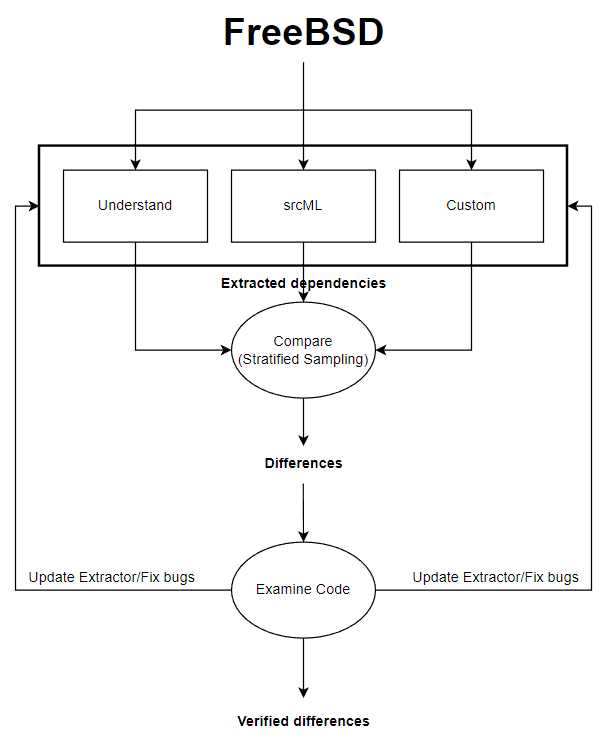
\includegraphics[width=200pt]{assets/qualitative_process_diagram.PNG}
	\caption{Qualitative Comparison's Process Diagram}
\end{figure}
This is the process of our qualitative comparison. After obtaining the extracted dependencies from each technique, we applied the Stratified Sampling to get samples. Here, the population is the union set of all the techniques minus the common dependencies, which is equivalent to 205,963.
By utilizing a calculator from Creative Research Systems \cite{calculator}, we got 383 as a needed sample size. We divided all the dependencies into 7 stratas and fetched the appropriate number of dependencies from them.
For example, the number of dependencies extracted only by our Custom method is 8, and the proportion of the stratum is 8 divided by 205,963, which is approximately 0.000039.
That is, the sample size needed for the particular stratum is 383 multiplied by 0.000039, which is approximately 0.
After completing all the calculations, we obtained 270 samples from dependencies which only Understand extracted and 113 samples from the common dependencies, extracted by both Custom and srcML methods.
Moreover, we fetched a single random dependency from the other stratas to introduce more variety of reasons for the existence of dependencies in each strata.
After the Stratified Sampling, we observed each dependency to find any differences, examined its file code, and updated our extractors when necessary. We repeated these steps until we classified all the dependencies.
\subsection{Results of Qualitative Comparison}
\subsubsection{Comparison Between Understand and Custom}
\underline{Understand-Only Dependencies}
\newline
\newline
Example$\,\colon\,$\texttt{freebsd/sys/fs/nfsclient/nfs\_clsubs.c \\$\,\to\,$ freebsd/sys/fs/nfsclient/nfs.h}
\newline
\newline
This dependency was extracted because this \texttt{nfs\_clsubs.c} file includes \texttt{nfs.h} as an imported file. Only Understand was able to fetch this dependency as our Custom script is built to fetch the first match, which results in capturing \texttt{nfs.h} under \texttt{sontib/tcpdump} folder.

\underline{Custom-Only Dependencies}
\newline
\newline
Example$\,\colon\,$\texttt{freebsd/sys/dev/pms/RefTisa/sallsdk/spc/sahw.c \\$\,\to\,$ freebsd/sys/dev/pms/RefTisa/sallsdk/hda/64k/iopimg.h}
\newline
\newline
The dependency is found here because ioparray within \texttt{iopimg.h} is included and utilized in \texttt{sahw.c}.
However, Understand did not include this dependency as the used location is within a comment line but within the actual run code. Therefore, it was assumed by Understand that it is an unnecessary dependency to extract.

\underline{Common Dependencies Between Understand And Custom}
\newline
\newline
Example$\,\colon\,$\texttt{freebsd/sys/dev/pms/freebsd/driver/ini/src/agtiapi.c \\$\,\to\,$ freebsd/sys/cam/cam\_sim.h}
\newline
\newline
\texttt{cam\_sim.h} is included and utilized in \texttt{agtiapi.c} for creating structs. For this dependency, Understand simply extracted it, and the Custom script also extracted it without any issues as \texttt{cam\_sim.h} with this particular file name can be found only once in the system.
\clearpage
\subsubsection{Comparison Between Understand and srcML}
\underline{Understand-Only Dependencies}
\newline
\newline
Example$\,\colon\,$\texttt{freebsd/sys/contrib/libnv/cnvlist.c \\$\,\to\,$ freebsd/sys/sys/nv.h}
\newline
\newline
For this Understand-only dependency, \code{cnvlist.c} uses data structures and functions defined in \code{nv.h}. \code{nv.h} is a header file that defines the "name-value" (NV) pair data structure. The \code{cnvlist.c} source file in \code{libnv} provides functions for creating, manipulating, and storing NV pairs.

Example$\,\colon\,$\texttt{freebsd/sys/contrib/dev/acpica/compiler/aslmaputils.c \\$\,\to\,$ freebsd/sys/contrib/dev/acpica/include/acobject.h}
\newline
\newline
Although not a direct dependency understand was able to still catch indirect dependencies between these files. \code{acobject.h} is a header file that defines various ACPI object data structures and functions used throughout the ACPI subsystem. The \code{aslmaputils.c} source file provides utilities for mapping ACPI names to objects and vice versa, as well as for searching and validating ACPI namepaths.

\underline{srcML-Only Dependencies}

Example$\,\colon\,$\texttt{freebsd/sys/dev/cfe/cfe\_resource.c \\$\,\to\,$ freebsd/contrib/sendmail/include/sm/cdefs.h}
\newline
\newline
The reason for the apparent dependency between these two files is that \code{cfe\_resource.c} includes a header file that is defined in \code{cdefs.h}.


\underline{Common Dependencies Between Understand And srcML}
\newline
\newline
Example$\,\colon\,$\texttt{freebsd/sys/dev/smartpqi/smartpqi\_event.c \\$\,\to\,$ freebsd/sys/dev/smartpqi/smartpqi\_includes.h}
\newline
\newline
The \code{smartpqi\_event.c} source file in the \code{smartpqi} driver for FreeBSD includes the \code{smartpqi\_includes.h} header file because it contains various data structures and function declarations declared in \code{smartpqi\_includes.h}. \code{smartpqi\_includes.h}  provides definitions for the data structures used to represent various events that can occur in the driver.


\subsubsection{Comparison Between Custom and srcML}
\underline{Custom-Only Dependencies}
\newline
\newline
Example$\,\colon\,$\texttt{freebsd/sys/dev/pms/RefTisa/sallsdk/spc/sahw.c \\$\,\to\,$ freebsd/sys/dev/pms/RefTisa/sallsdk/hda/64k/iopimg.h}
\newline
\newline
It is the same dependency as the one, brought up earlier for the comparison between Understand and Custom. As well as Understand, srcML also ignored the dependency as \texttt{iopimg.h} was included within commented-out lines.

\underline{srcML-Only Dependencies}
\newline
\newline
Example$\,\colon\,$\texttt{artpqi/smartpqi\_event.c \\$\,\to\,$ freebsd/sys/dev/smartpqi/smartpqi\_includes.h}
\newline
\newline
For this srcML-only dependency, this was included only in a srcML extracted list, and the reason for this was due to the missing white space in include reference.

\underline{Common Dependencies Between Custom And srcML}
\newline
\newline
Example$\,\colon\,$\texttt{freebsd/sys/dev/beri/virtio/network/if\_vtbe.c \\$\,\to\,$ freebsd/sys/amd64/include/cpu.h}
\newline
\newline
For this dependency, we were not able to find a clear rationale. Because both Custom and srcML contain this sample, we first assumed that \texttt{if\_vtbe.c} includes \texttt{cpu.h}. However, after examination, we found out that the \texttt{if\_vtbe.c} imports \texttt{cpu.h}, but not in the path shown in the list of extracted dependencies. Instead, the imported \texttt{cpu.h} was under a \texttt{machine} folder.
Because the file location is still under the \texttt{machine} folder within a XML file we obtained, we assume that the srcML script we created might need to be modified to show the correct path.
\clearpage

\subsubsection{Performance Metrics}
For the Performance metrics, we utilized recall and precision for our Custom and srcML by including Understand as Oracle.
Here, we have two formulas to calculate recall and precision. As well as these formulas, we included a diagram which shows which dependency sets we examined to obtain solutions.

\begin{equation*}
	\begin{split}
		Recall &= \frac{True Positive}{(True Positive + False Negative)}
	\end{split}
\end{equation*}
\newline
\begin{equation*}
	\begin{split}
		Precision &= \frac{True Positive}{(True Positive + False Positive)}
	\end{split}
\end{equation*}

\begin{figure}[h]
	\center
	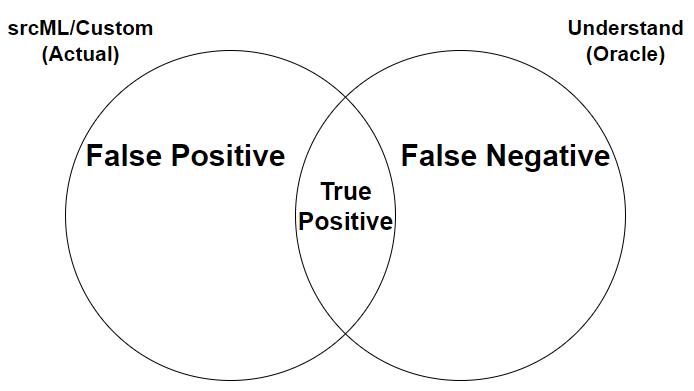
\includegraphics[width=300pt]{assets/recall_precision_diagram.PNG}
	\caption{Classification Diagram}
\end{figure}

For both Custom and srcML, we obtained the same results shown below$\,\colon\,$
\newline
For recall, we obtained 66 True Positive dependencies and 270 False Negative dependencies.
\begin{equation*}
	\begin{split}
		Recall &= \frac{66}{(66 + 270)}\\
		&= 0.196428571\dots\\
		&\approx 20\%
	\end{split}
\end{equation*}
For precision, we obtained the same number of True Positive dependencies and 133 False Positive dependencies.
\begin{equation*}
	\begin{split}
		Precision &= \frac{0 + 66}{(66 + 113)}\\
		&= 0.3687150\dots\\
		&\approx 37\%
	\end{split}
\end{equation*}
\clearpage

\section{Limitations \& Recommendations}
Code analysis tools, both static and dynamic, play an essential role in software development. They help identify issues in code, improve code quality, and increase the overall reliability of software. However, like all tools, they have limitations. We will now discuss the limitations of Understand, SrcML, and our custom analysis. We will also recommend how we could have improved the process if we had more time to explore other dependency extraction techniques. Code analysis tools are essential in software development but have limitations since dependency extraction is non-trivial. Understanding the limitations of these tools is crucial to use them to extract dependencies effectively.

\subsection{Limitations of SrcML and Custom}
The SrcML and custom methods have similar limitations as they extract "include" directive dependencies. For our custom method, the regular expression used to find the include directives in source files is simple and may only capture some possible include statement formats. For example, \code{\#include"test.h"} will not be matched as it is a missing edge case for the space after the include directive. The script also assumes that all files with a "\code{.c}," "\code{.cpp}," or "\code{.h}" extension are C or C++ source files, which may not be accurate in all cases and could result in incorrect or missing dependencies in other types of projects. One of our most significant limitations was extracting the correct include file path. The SrcML and custom method exit early after finding the first match of a header file. This limitation introduces false positives in the case multiple directories have the same header file.

Furthermore, the scripts do not handle circular dependencies between files, and it only looks for header files in directories containing C or C++ source files. Additionally, these include methods do not account for conditional compilation directives, such as \code{\#ifdef} and \code{\#ifndef}, which could result in missing or incorrect dependencies. Lastly, these include methods do not handle call graph dependencies and other types of dependencies, which is evident in our reduced extracted dependencies compared to Understand.

The SrcML and custom method are similar, as seen by our performance metrics and quantitative analysis. The include method is generally less effective than how Understand processes dependencies, as Understand had a significantly more significant number of mutually-exclusive dependencies that the include methods could not find due to the limitations.

\subsection{Understand}
The Understand static code analysis tool also has limitations despite being a robust commercial tool. One of the primary limitations is a high false-positive rate, and understanding sometimes identifies dependencies that are not in the source code, leading to a high false-positive rate. Additionally, while Understand supports a wide range of programming languages, it may only support some features, making it challenging to analyze code that uses those features.

Furthermore, Understand cannot analyze dynamic code since it is a static code analysis tool. This means it cannot analyze dynamic code or code generated at runtime. Lastly, Understand can be resource-intensive and time-consuming when analyzing large codebases, making it challenging to use on large projects and may impact its effectiveness.

\subsection{Recommendations}
If we had more time, one way to improve these limitations would be to explore other dependency extraction techniques, such as compiling the source code and extracting linked library dependencies instead of using two methods that include directives. Alternatively, we can expand using SrcML and create a custom parser that generates a call graph based on XPath queries on the XML function units.
\clearpage

\section{Conclusion}
To conclude, based on the results and observations presented, it is clear that the choice of dependency extraction tool can have a significant impact on the number and types of dependencies identified in a codebase. Understand appears to be the most thorough and comprehensive tool, identifying over 180,000 dependencies, 80\% of which were exclusive to that tool. However, it is worth noting that this may lead to more false positives or irrelevant dependencies being identified. srcML and the custom script both focused primarily on include files and identified around 96,000 dependencies, with srcML having no exclusive dependencies and the custom script having only 8. The similarity in their statistics suggests that they may have similar strengths and limitations.

The observation that Understand analyses dependencies based on functions calling other functions while srcML and the custom script prioritize "include" files only suggests that the former may be more effective at identifying dynamic or runtime dependencies, while the latter may be more appropriate for identifying static or compile-time dependencies. However, it is important to note that both types of dependencies can be important in understanding the architecture of a codebase.

In terms of choosing a methodology for dependency extraction in FreeBSD, the specific goals and characteristics of the analysis should be taken into account. For example, if the goal is to identify dynamic dependencies, Understand may be the most appropriate tool. If the focus is on static dependencies based on include files, srcML or the custom script may be more effective. However, it is worth noting that no single tool or methodology may be sufficient on its own, and a combination of techniques may be needed for a more comprehensive understanding of the architecture.

Overall, the process of extracting and analyzing architectural dependencies in FreeBSD can be complex and may require careful consideration of the specific needs of the analysis. The tools and methodologies used should be chosen based on the specific goals of the analysis and the characteristics of the codebase being analyzed. By taking these factors into account and combining multiple techniques as necessary, a more complete understanding of the architecture of FreeBSD can be achieved.

\section{Lessons Learned}
The importance of choosing the right tool: The choice of tool for dependency extraction can have a significant impact on the results and effectiveness of the analysis. It is important to carefully consider the strengths and limitations of each tool and select the one that is most appropriate for the specific goals and characteristics of the analysis.

The importance of understanding the codebase: A thorough understanding of the codebase is crucial for effective dependency extraction and analysis. Without a good understanding of the code structure, it can be difficult to interpret the results and identify relevant dependencies.

The value of combining multiple techniques: While each tool or methodology may have its own strengths and limitations, combining multiple techniques can provide a more comprehensive understanding of the architecture. For example, using both Understand and a custom script may help to identify both dynamic and static dependencies.

The risk of false positives and irrelevant dependencies: Some tools may identify a large number of dependencies, many of which may not be relevant to the specific analysis. It is important to carefully review and validate the results to avoid being misled by false positives or irrelevant dependencies.

The need for ongoing analysis and refinement: As codebases evolve over time, the architecture and dependencies may change as well. Ongoing analysis and refinement of the dependency extraction process is needed to ensure that the results remain accurate and relevant. This may involve updating the tools and techniques used, as well as revisiting the goals and objectives of the analysis.
\clearpage
\section{Data Dictionary}
\begin{itemize}
	\item{Stratified Sampling: A sampling technique which divides the whole dependency set into multiple strata based on their number proportion}
	\item {SrcML: A light weight tool to transform and analyze source code in XML format}
	\item {XPath: A query syntax to perform syntactic analysis on SrcML generated XML}
	\item {Oracle: A source of comparison, in this case Understand dependency extraction}
	\item {False Positive: Dependency that was incorrectly identified as present}
	\item {False Negative: Dependency that was incorrectly identified as not present}
	\item {True Positive: Dependency that was correctly identified as present}
\end{itemize}

\section{Naming Conventions}
\begin{itemize}
	\item {XML: Extensible Markup Language}
	\item {IDE: Integrated Development Environment}
	\item {CSV: Comma Separated Values}
\end{itemize}

\begin{thebibliography}{00}
	\bibitem{b2} Clarke, Arthur C. 2001: A Space Odyssey. New York: Roc, 1968. 297.
	\bibitem{sourcecode} “BitTheory A3 source code.” README.md, \href{https://github.com/BitTheoryProject/eecs4314-reports/tree/main/a3/src}{https://github.com/BitTheoryProject/eecs4314-reports/tree/main/a3/src}.
	\bibitem{understand} “BitTheory A2 Understand steps.” README.md, \href{https://github.com/BitTheoryProject/eecs4314-reports/tree/main/a2/src}{https://github.com/BitTheoryProject/eecs4314-reports/tree/main/a2/src}.
	\bibitem{calculator} “Sample Size Calculator.” Sample Size Calculator \- Confidence Level, Confidence Interval, Sample Size, Population Size, Relevant Population \- Creative Research Systems, 2012, \href{https://www.surveysystem.com/sscalc.htm}{https://www.surveysystem.com/sscalc.htm}.
	\bibitem{srcml} “SrcML Documentation .” \href{https://www.srcml.org/documentation.html}{https://www.srcml.org/documentation.html}.
\end{thebibliography}
\end{document}
